% Source of the figure worked-example.pdf: the graph G_1 (vertices u, v, 1, ..., 8) with its square decomposition for
% the pair (u,v). F = all edges except 12, 13, 23, 67, drawn from tail to head; squares S_1 = {u}, S_2 = {1,2,3},
% S_3 = {6,7}, S_4 = {v}; links {4}, {5}, {8}. Compile with pdfLaTeX; the PDF is included in the manuscript at its
% natural size.
\documentclass[tikz,border=1pt]{standalone}
\usepackage[T1]{fontenc}
\pdfinfoomitdate=1 \pdftrailerid{} \pdfsuppressptexinfo=-1
\usetikzlibrary{arrows.meta,shapes.geometric}
\definecolor{fblue}{RGB}{31,102,178}
\tikzset{
  vertex/.style={circle, fill=black, inner sep=0pt, minimum size=2.2mm},
  terminal/.style={circle, fill=black, inner sep=0pt, minimum size=3mm},
  edge/.style={line width=0.7pt},
  square/.style={rounded corners=4pt, fill=gray!14, draw=gray!75!black, line width=0.9pt},
  link/.style={ellipse, fill=gray!32, draw=gray!75!black, line width=0.6pt, inner sep=0pt,
               minimum width=9mm, minimum height=7mm},
  fedge/.style={line width=0.9pt, fblue, dash pattern=on 3pt off 1.6pt, -{Stealth[length=2.4mm, width=2mm]}}}
\begin{document}
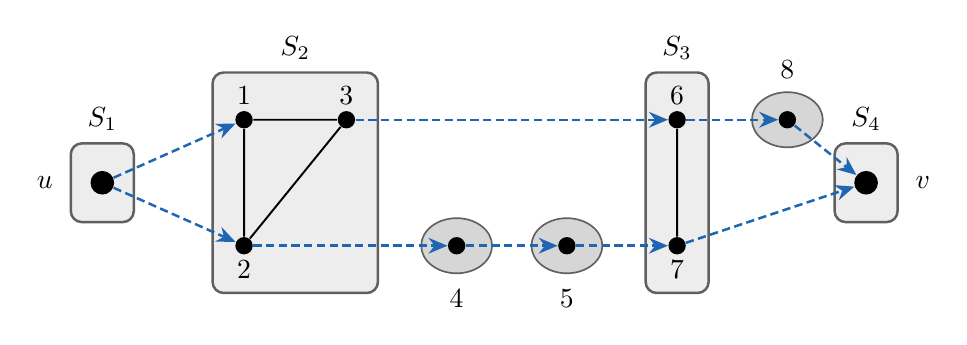
\begin{tikzpicture}[x=1cm, y=1cm]
  % pieces
  \draw[square] (-0.4,-0.5) rectangle (0.4,0.5);
  \draw[square] (1.4,-1.4) rectangle (3.5,1.4);
  \draw[square] (6.9,-1.4) rectangle (7.7,1.4);
  \draw[square] (9.3,-0.5) rectangle (10.1,0.5);
  \node[above=1pt] at (0,0.5)    {$S_1$};
  \node[above=1pt] at (2.45,1.4) {$S_2$};
  \node[above=1pt] at (7.3,1.4)  {$S_3$};
  \node[above=1pt] at (9.7,0.5) {$S_4$};
  \node[link] (l4) at (4.5,-0.8) {};
  \node[link] (l5) at (5.9,-0.8) {};
  \node[link] (l8) at (8.7,0.8)  {};
  % vertices
  \node[terminal] (u) at (0,0)      {};
  \node[terminal] (v) at (9.7,0)   {};
  \node[vertex] (n1) at (1.8,0.8)   {};
  \node[vertex] (n2) at (1.8,-0.8)  {};
  \node[vertex] (n3) at (3.1,0.8)   {};
  \node[vertex] (n4) at (4.5,-0.8)  {};
  \node[vertex] (n5) at (5.9,-0.8)  {};
  \node[vertex] (n6) at (7.3,0.8)   {};
  \node[vertex] (n7) at (7.3,-0.8)  {};
  \node[vertex] (n8) at (8.7,0.8)   {};
  \node[left=3pt]  at (-0.4,0)  {$u$};
  \node[right=3pt] at (10.1,0)  {$v$};
  \node[above=2pt] at (n1) {$1$};
  \node[below=2pt] at (n2) {$2$};
  \node[above=2pt] at (n3) {$3$};
  \node[below=2pt] at (l4.south) {$4$};
  \node[below=2pt] at (l5.south) {$5$};
  \node[above=2pt] at (n6) {$6$};
  \node[below=2pt] at (n7) {$7$};
  \node[above=1pt] at (l8.north) {$8$};
  % edges outside F
  \draw[edge] (n1) -- (n2) (n1) -- (n3) (n2) -- (n3) (n6) -- (n7);
  % edges of F, from tail to head
  \draw[fedge] (u) -- (n1);
  \draw[fedge] (u) -- (n2);
  \draw[fedge] (n3) -- (n6);
  \draw[fedge] (n2) -- (n4);
  \draw[fedge] (n4) -- (n5);
  \draw[fedge] (n5) -- (n7);
  \draw[fedge] (n6) -- (n8);
  \draw[fedge] (n8) -- (v);
  \draw[fedge] (n7) -- (v);
\end{tikzpicture}
\end{document}
